\documentclass[10pt,twocolumn]{article}
\usepackage[top=0.5in,bottom=0.7in,left=0.5in,right=0.5in]{geometry}
\setlength{\parskip}{0in}
\setlength{\parskip}{1ex plus 0.5ex minus 0.2ex}
\usepackage{graphicx}
\usepackage{subfigure}
\begin{document}
\sloppy

\onecolumn

\begin{center}
  {\bf Evaluation of linear interpolation for SHOC} \\
  E3SM/SCREAM (\today)
\end{center}

\noindent {\bf Motivation.}

The SHOC code is currently being incorporated into SCREAM and will soon be ported to
C++. The fortran version contains a linear interpolation routine that is using a
sub-optimal quadratic algorithm for finding the nearest point in the second coodinate
space. SHOC performs several linear interpolations per time step, so we need to
use a better algorithm.

We have set up a ``micro-app'' to develop, test, and performance-test a linear
iterpolation routine that will be performant and generally useful to all C++ SCREAM
code.

\noindent {\bf Implementation}

We broke up the algorithm into two phases, an O($n \log n$) setup phase and the actual
O($n$) linear interpolation. The setup phase creates a map, for each x2 coordinate, to
the nearest x1 coordinate. The idea here is that a user can do the setup phase once, and
then do several linear interpolations (assuming they use the same coodinates). The more
linear interpolations that are done per setup, the better the performance, but the algorithm
is still optimal even if only one linear interpolation is done.

We wrote two implementations (other than the fortran reference implementation) of our
algorithm. One (li\_kokkos) that is a basic C++/Kokkos implementation of the algorithm
described above and one (li\_vect) that attempts to add vectorization to the basic implementation.

li\_kokkos was very straightforward, but li\_vect was a bit trickier. The most interesting
vectorization exercise was turning this:


\begin{verbatim}
    Kokkos::parallel_for(Kokkos::TeamThreadRange(team, lik.m_km2), [&] (Int k2) {
      const int k1 = lik.m_indx_map(i, k2);
      ...
        y2(k2) = y1(k1) + (y1(k1+1)-y1(k1))*(x2(k2)-x1(k1))/(x1(k1+1)-x1(k1));
      ...
\end{verbatim}

into this

\begin{verbatim}
Kokkos::parallel_for(Kokkos::TeamThreadRange(team, liv.m_km2_pack), [&] (Int k2) {
      const auto indx_pk = liv.m_indx_map(i, k2);
      ...
        Pack x1p, x1p1, y1p, y1p1;
        scream::pack::index_and_shift<1>(x1s, indx_pk, x1p, x1p1);
        scream::pack::index_and_shift<1>(y1s, indx_pk, y1p, y1p1);
        const auto& x2p = x2(k2);

        y2(k2) = y1p + (y1p1-y1p)*(x2p-x1p)/(x1p1-x1p);
      ...
\end{verbatim}

We were able to do the common-case linear interpolation without needing scalarized
views. This required the index\_and\_shift function, which looks-up two packs-worth
of data, one using indx\_pk and one using indx\_pk with each index shifted by a known
compile-time constant, which should be generally useful.

\noindent {\bf Correctness testing}

We do BFB checks against the fortran reference for predefined full runs, but our best test is
li\_unit\_test, which is a ``soak'' test that populates x1, x2, and y1 with random
values and randomizes km1 and km2 as well. We do 1000 of these randomized tests,
ensuring both our implementations are producing the same result as the fortran reference.

I've leveraged our gather-all-data script to distribute the tests described above to four different
archictectures (HSW, KNL, SKX, and V100).

\noindent {\bf Performance testing}

Linear interpolation is very fast for realistic input data (128 levels, 2048 columns), so we
had to leverage a lot of repetition to reduce noise. Our drivers were instrumented to support
internal repetitions (run code-of-interest within an N-loop, then divide walltime by N) and our performance scripts
support external repetitions (run executable M times, then take median). I settled on
200x20 repetitions (200 internal run 20 times) as a value that ran quickly and eliminated
most noise.

Instrumentation was also added so we could test the setup cost instead of the li cost
if desired.

We populate a single column with random inputs (consistent seed) and then replicate it
across all columns.

\noindent {\bf Results/Conclusion}

The scalar implementation, li\_kokkos, auto-vectorizes,
as is evident for example by outputting readable assembly with the Intel compiler arguments {\tt -S -fsource-asm}.
Thus, unlike in the sedimentation micro-app, but similar to the tridiagonal solver nano-app,
the pack-based implementation competes against auto-vectorized code.
On SKX, li\_vect is slower than li\_kokkos;
on KNL, it is faster.
The explanation is that the auto-vectorization produces assembly that use vector registers and instructions smaller than 512 bit.
These essentially always lead to suboptimal performance on KNL relative to perfectly vectorized (via packs) 512-bit instructions.
In contrast, on SKX, CPU cycle throttling and other complexities make for complicated trade offs. 
However, the {\tt Pack} implementation compiles away to simple scalar operations when the pack size is set to 1;
this setting makes li\_vect and li\_kokkos perform nearly the same on SKX.
Here we use the performance-portability aspect of the design of SCREAM.

We were also not able to get KNL to perform as well as SKX. TODO
%todo I think this is true only for small problems, where for this simple problem, SKX is keeping data in probably L2 and certainly L3. For a sufficiently large problem, KNL ought to pull even with SKX b/c its 16 GB of high b/w memory will outperform an out-of-L3 run on SKX. If you confirm this, I recommend making an extra figure that shows this for KNL, SKX, and V100. This way, even though it's not a practically useful result, we can at least explain what's happening.

For linear interpolation only, see figure 1. V100 scales best since it has so much more parallelism
available. KNL gets a nice speedup with packs (vectorization) but is still about 2x slower than SKX
for our largest runs. SKX performance of li\_kokkos and li\_vect is nearly exactly the same, which is
expected since we're using packsize=1 on SKX. This at least shows that the pack implementation does not incur
any extra overhead.

For setup cost only, see figure 2. Both SKX and KNL tail off quickly since this is a nlogn algorithm. V100
again scales great since, even at 8192 columns, it can give a cuda thread to each vertical level in every
column. KNL does not get much benefit from vectorization since we have to scalarize the x1 coords in order
to do the binary-search for the x1 coord that is closest to the current x2 coord.

For total perf, see figure 3. For this test, we only did one interpolation per setup. We show
the performance for the fortran reference implementation. SKX and KNL are dominated by setup
time. We get a 3x speedup on SKN and KNL compared to the fortran reference. There is no fortran
reference for V100 since we did not add CUDA support to it.

\onecolumn

\begin{figure}[hbt]
  \centering
  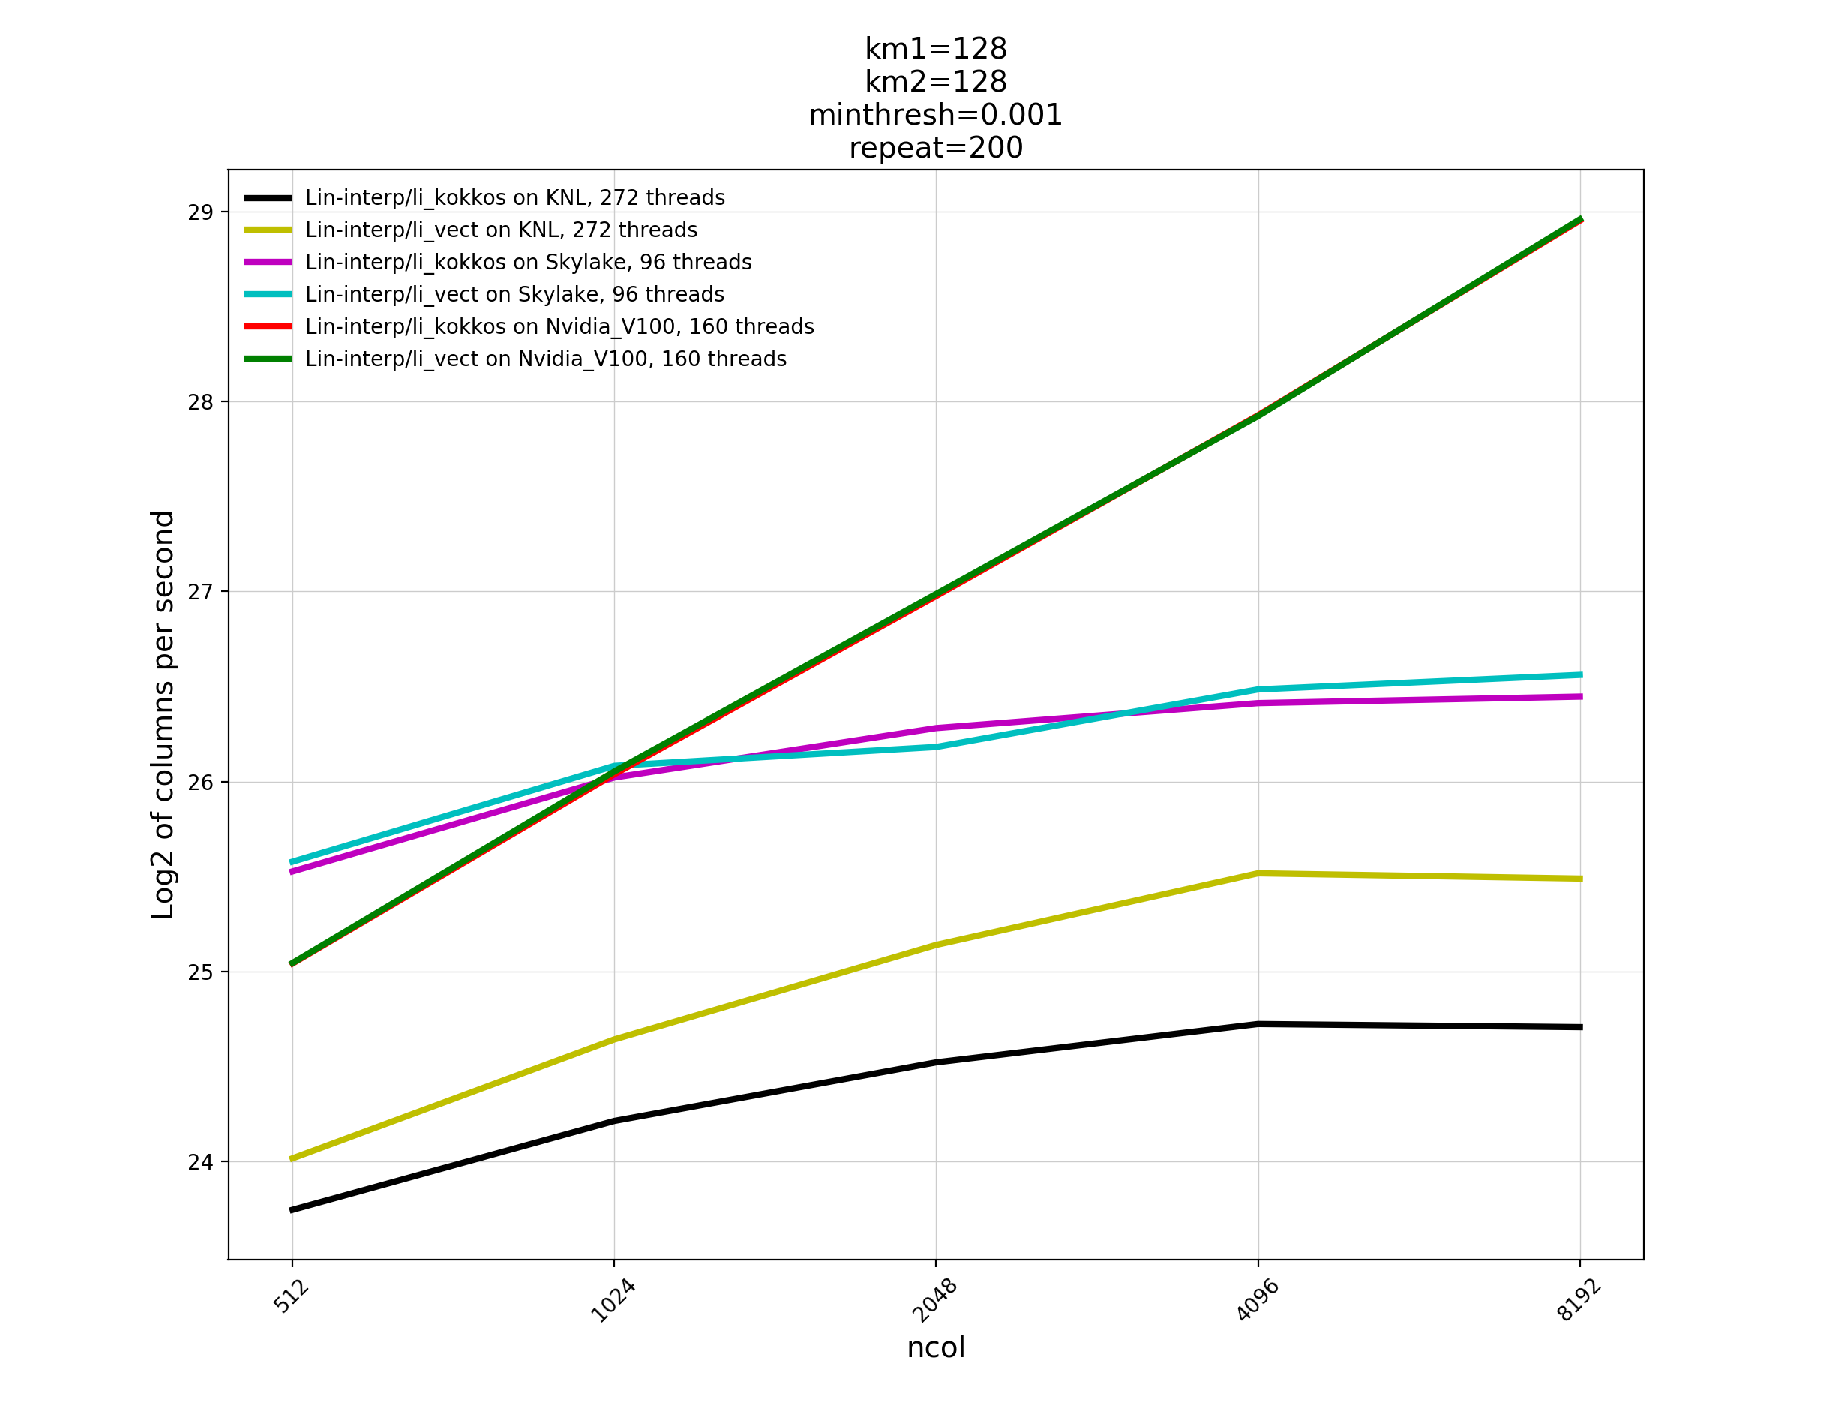
\includegraphics[width=1.0\linewidth]{final-li.pdf}
\end{figure}

\begin{figure}[hbt]
  \centering
  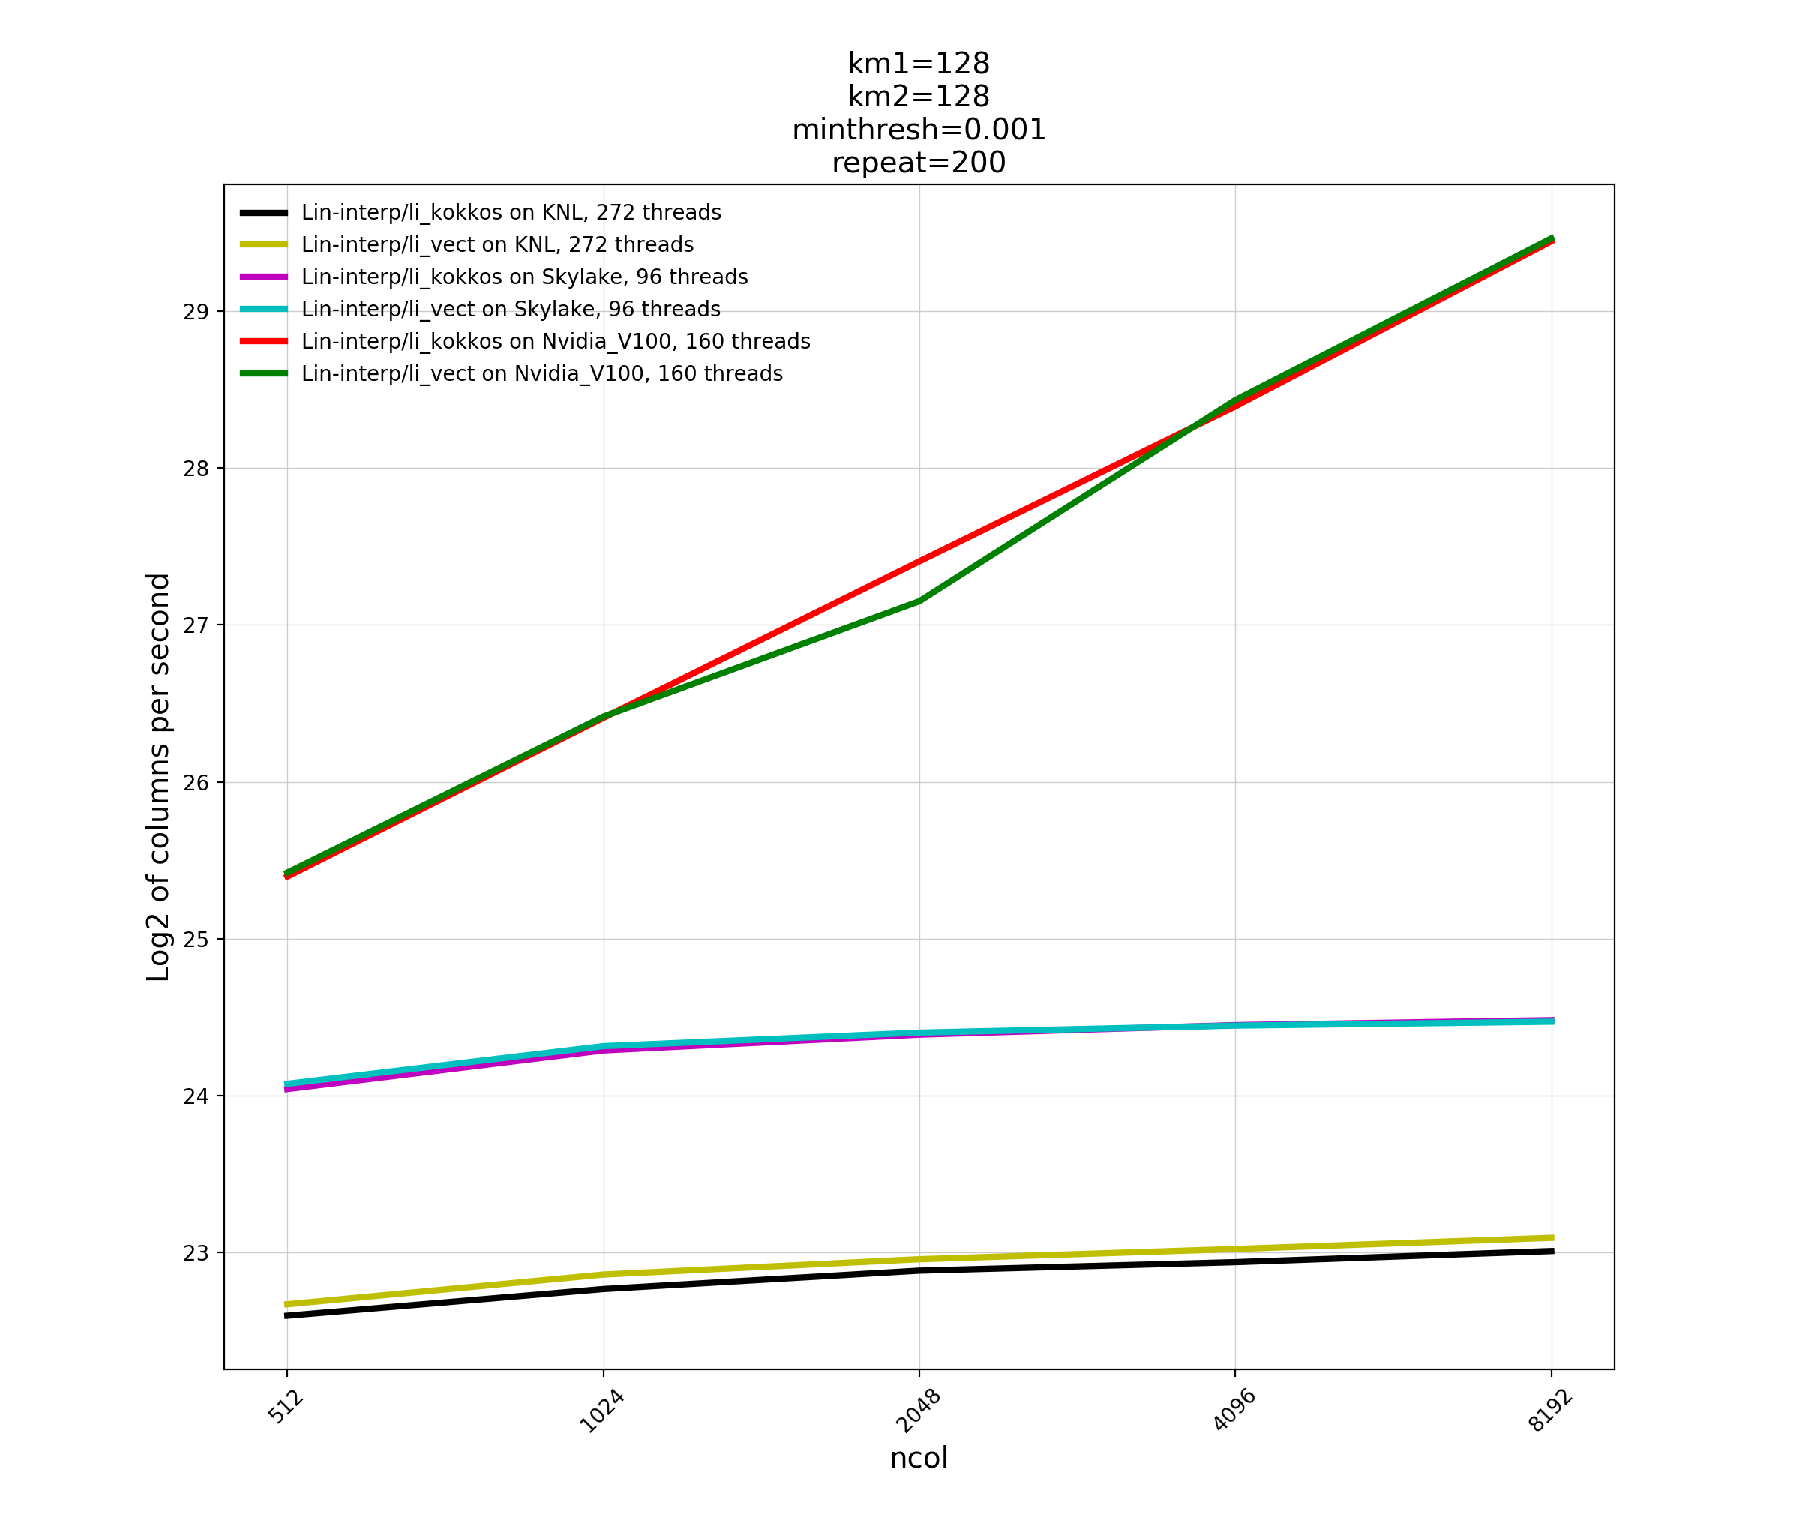
\includegraphics[width=1.0\linewidth]{final-setup.pdf}
\end{figure}

\begin{figure}[hbt]
  \centering
  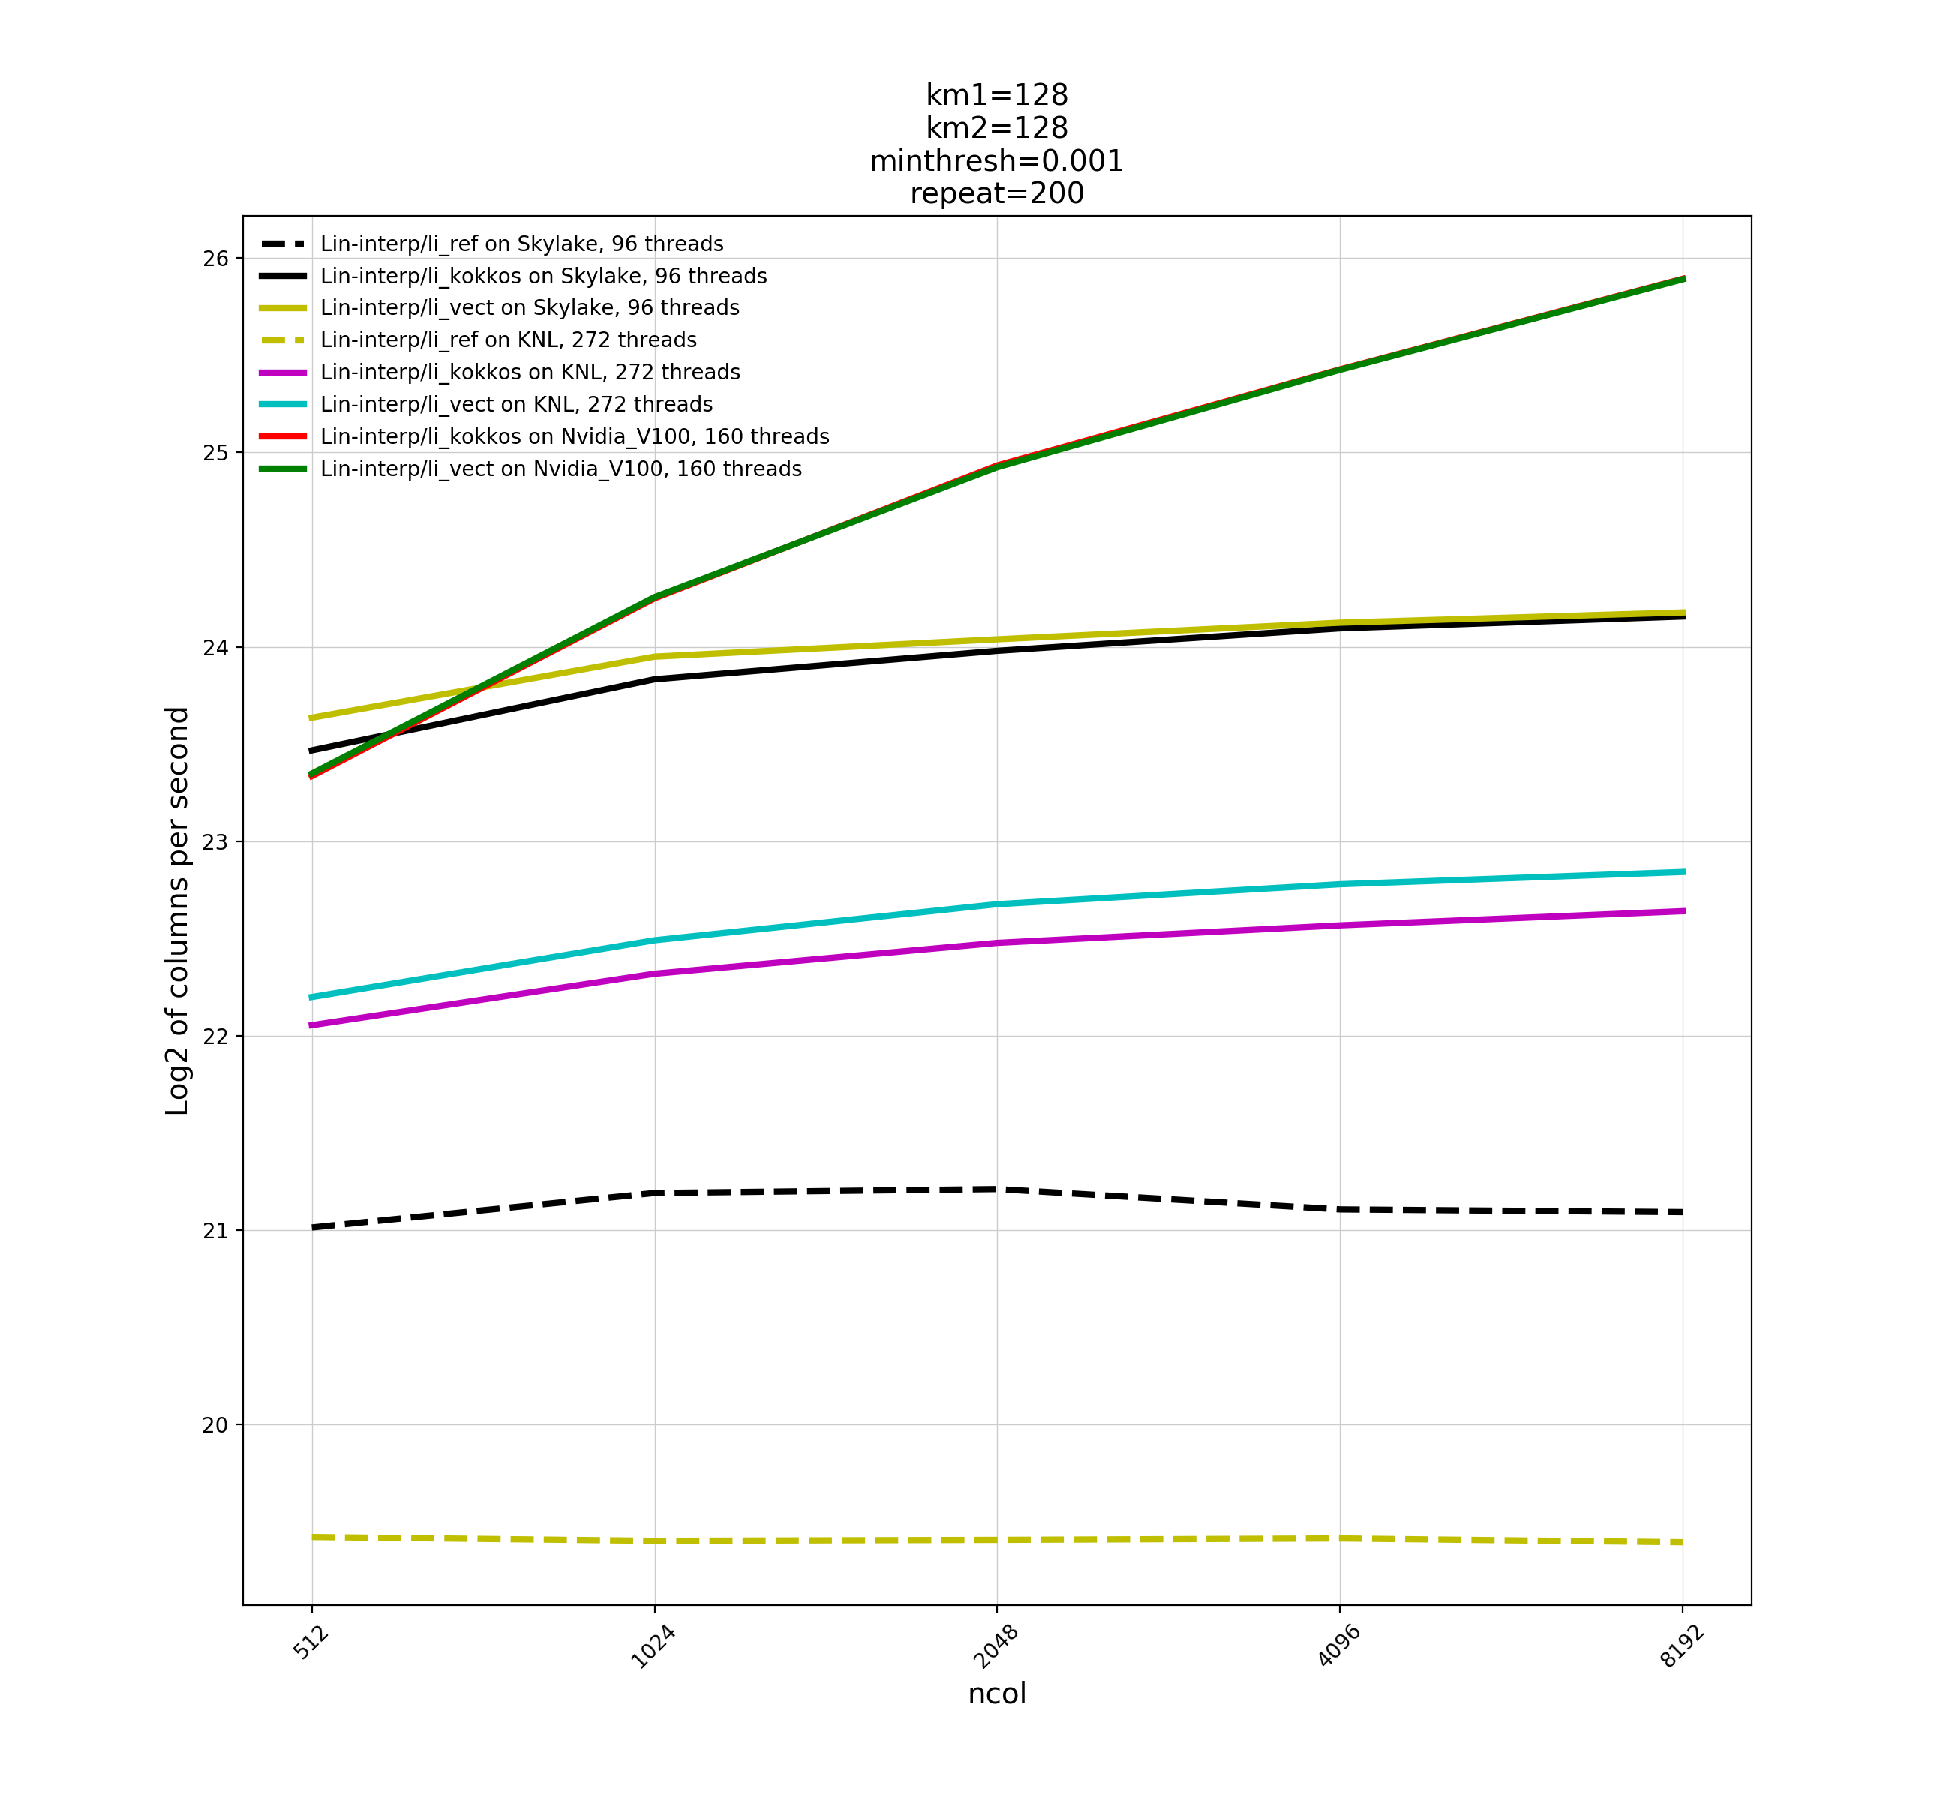
\includegraphics[width=1.0\linewidth]{final-total.pdf}
\end{figure}

\end{document}
